\section{Blind Test \aha}

\subsection{\ah Arena}

\ah est le premier gérant d'hôtel de France et le 6e mondial.
À l'occasion d'un partenariat, le Palais omnisports de Paris-Bercy s'est vu renommé \aha pour 10 ans.

Le site accueillant beaucoup de concerts et de spectateurs, \ah a voulu communiquer au travers d'une installation interactive.
Cette installation est un quizz musical (ou \emph{Blind test}) composé d'un écran et d'un iPad permettant de saisir les réponses.

Le jeu est simple : une chanson est jouée sur l'écran et le titre de cette chanson est indiqué.
Le joueur dispose alors de 45 secondes pour trouver l'artiste en question parmi les quatre proposés.
On enchaîne ainsi sur six questions qui se terminent sur le résultat du jeu affiché à l'utilisateur.

\subsection{Technologies}

Les technologies utilisées dans ce projet sont standards et étaient déjà maîtrisées par les membres de l'équipe.
On retrouve alors une application \emph{Electron} pour l'affichage sur l'écran et un serveur NodeJS avec le framework \emph{Express} pour servir les fichiers et gérer le jeu.
Enfin, on utilise \emph{Socket.io} pour les WebSockets apportant de l'interactivité.

\subsubsection{Express}

Express est une librairie utilisant les capacités de NodeJs (inclus dans \emph{Electron}) à mettre en place un serveur Web.
Express permet de répondre à une URL, mais aussi de servir des fichiers en tout genre.

Nous avons choisi Express car il est léger et simple à mettre en place.
Il dispose d'une grande communauté et permet de mettre en place un serveur Web et websocket rapidement.

Nous n'avions pas besoin ici d'une solution plus lourde car les seules interactions HTTP sont les demandes de médias comme la musique et les images ou la demande de page WEB.
Le reste des interactions s'effectuent au travers des Websockets.

\subsubsection{WebSockets}

La technologie de Websocket est un protocole Web de connexion bidirectionnel.
Il permet au serveur et au client de conserver une connexion TCP bidirectionnelle.

Ainsi il est possible au client d'envoyer des paquets arbitraires au serveur, mais aussi au serveur d'envoyer des paquets au client à n'importe quel moment.
Ainsi, il est possible de rendre l'application très interactive et dynamique.

Nous avons utilisé les WebSockets pour toute la communication entre le serveur et les clients (Écran et iPad) avec l'aide de Socket.io.
Cette librairie se place comme une surcouche aux websockets et reprend le principe d'événements de Nodejs.
En effet, elle met à disposition du développeur un objet \texttt{socket} agissant comme un émetteur et un récepteur d'événements.
Chaque événement est composé d'un nom et d'un objet de contexte.
Lors de l'émission, l'objet \texttt{socket} transmet l'événement et le contexte au client connecté.
Il est aussi possible de recevoir des événements et ainsi de communiquer de manière bidirectionnelle.

\subsection{Structure}

Le Blind Test se compose de trois éléments :

\paragraph{Le serveur Web} présent dans le processus principal de l'application Electron, il gère tout le jeu du début à la fin.
Il présente un serveur de fichiers permettant l'accès aux fichiers audio, aux fichiers d'image et aux pages Web depuis l'iPad et l'affichage.
Il dispose aussi d'un serveur WebSockets permettant une communication bidirectionnelle entre les clients (iPad et TV) et le serveur.

Ce serveur Web dispose d'un état définissant l'état actuel du jeu.
Cet état est transmis à tous les clients pour qu'ils actualisent leurs affichages lors d'un changement et de la connexion d'un nouveau client.

Le serveur Web construit en parallèle un objet Javascript \texttt{Game} contenant toutes les questions à poser, la question actuellement posée, les réponses des joueurs et le score.
Cet objet \texttt{Game} est transmis à chaque client lors de leur connexion ou lors du changement d'état du jeu.

Dès que l'état du jeu change, un événement socket.io est transmis à tous les clients connectés pour qu'ils actualisent leur affichage en fonction des données transmises par le serveur.

\paragraph{Les clients (TV et iPad)} Chacun charge une page HTML spécifique possédant un script spécifique.
Ce script va afficher le bon écran en fonction de l'état du jeu envoyé par le serveur et, éventuellement, demander une interaction à l'utilisateur.

Dès qu'un joueur tape sur une réponse, l'iPad envoie à son tour un paquet WebSocket au serveur pour qu'il l'enregistre et change d'état.
Le jeu continue alors jusqu'à ce que toutes les questions de tous les joueurs soient posées.

\begin{figure}[h]
    \centering
    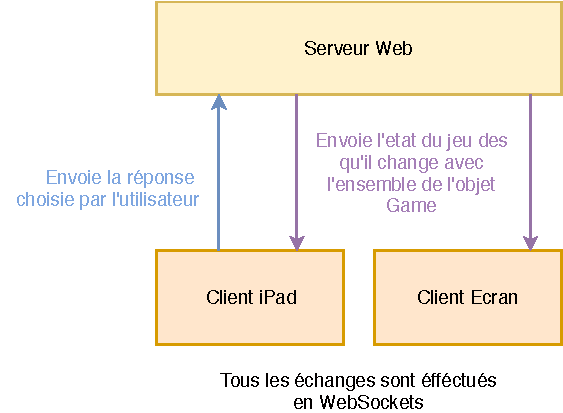
\includegraphics{img/ah-blindtest.pdf}
    \caption{Structure du jeu Blind Test}
\end{figure}

\subparagraph{TV} Coté TV, l'affichage est simple et permet d'afficher le score de l'utilisateur ainsi que de jouer la musique.
L'écran n'étant pas tactile, il ne permet que l'affichage d'informations sur l'état du jeu, mais aucune interactivité n'est possible directement.
Le client TV est une fenêtre de l'application Electron qui se connecte au serveur Express pour charger l'interface.

\subparagraph{iPad} Coté iPad, une application de kiosque permet d'afficher une page Web sans autre élément d'interface.
Cette page Web est chargée depuis le serveur et propose des choix à l'utilisateur en fonction de l'état du jeu.
Cela peut-être le nombre de joueurs, le nom de l'artiste en cours de lecture ou simplement une demande pour passer à la question suivante.

\subsubsection{Design}

Le design de l'application était fourni avec la demande du client et nous avons juste intégré ce design en extrayant des images clés du fichier Photoshop du designer.

\begin{figure}[h]
    \centering
    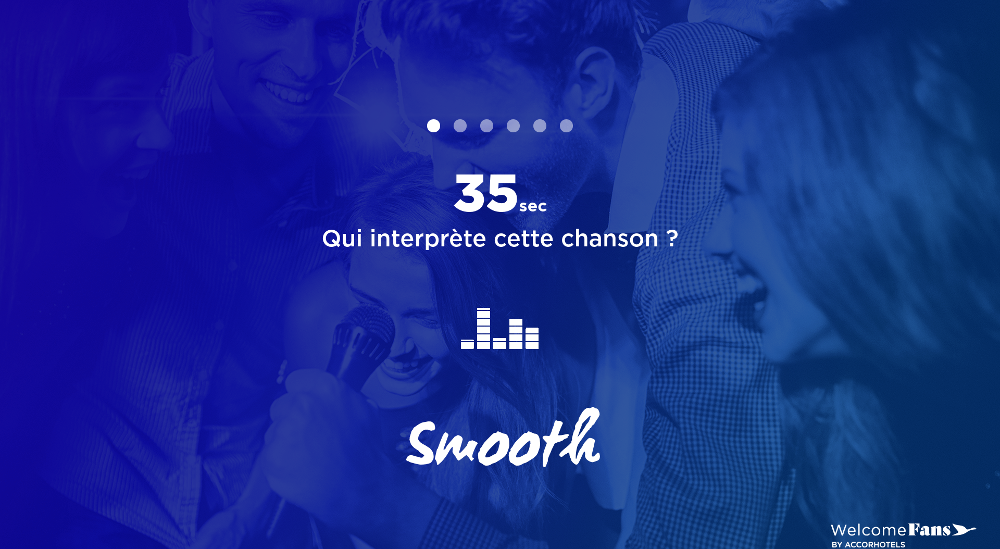
\includegraphics[scale=0.23]{img/blind-test-tv.png}
    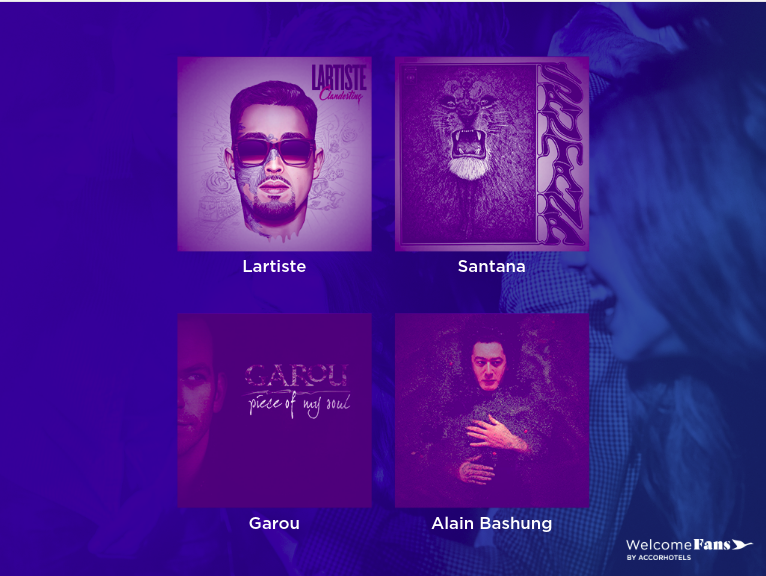
\includegraphics[scale=0.22]{img/blind-test-ipad.png}
    \caption{Une vue du Blind Test côté TV (à gauche) et côté iPad (à droite)}
\end{figure}

\subsubsection{Installation}

Je n'ai pas pu assister à l'installation du lundi 29 janvier, mais j'ai tout de même travaillé dessus à l'occasion de correction de bugs.

L'installation présente un grand écran connecté au serveur affichant l'interface TV sur une machine Windows hébergeant le serveur websocket que l'iPad pourra contacter.
On y retrouve bien évidemment L'iPad verrouillé pour éviter de sortir de l'application.
Ces deux terminaux sont connectés à une même borne WiFi permettant de disposer de son propre réseau évitant ainsi les latences dues à une éventuelle surcharge du réseau environnant.
Cette borne WiFi fait office de routeur vers l'extérieur, mais aussi de serveur DHCP et de point d'accès WiFi.

\begin{figure}[h]
    \centering
    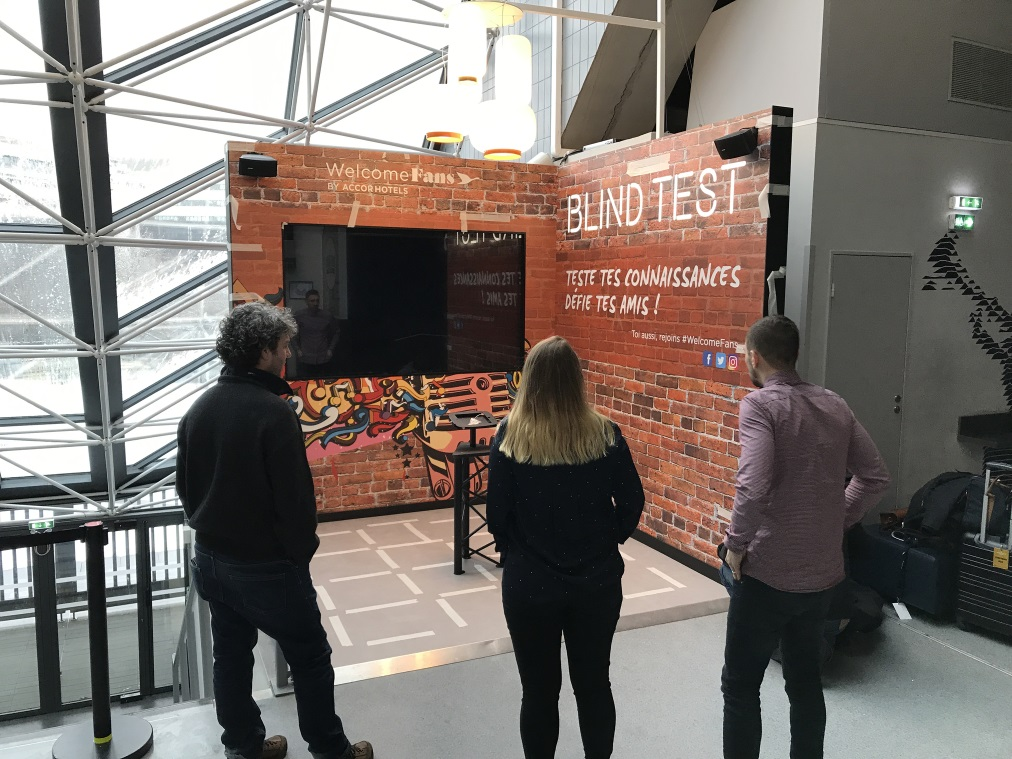
\includegraphics[scale=0.4]{img/accorhotel-blindtest-resize.jpg}
    \caption{Installation du Blind test à \aha}
\end{figure}

\subsubsection{Conclusion}

Ce projet fut intéressant et intense, car nous l'avons réalisé en seulement 2 jours.
Ce fut une bonne expérience de travail d'équipe et m'a permis de tester un projet à court délai.
Enfin, ce projet m'a permis de voir les techniques permettant de synchroniser l'état de multiples machines au travers de Websocket.
